\chapter{Results}\label{sec:results}
To verify both the correctness and the gain in terms of speed of execution of the new implementation of the bistable simulation engine many circuits has been simulated both with cpu and gpu.
As already said the parameters that mainly affect simulation time are the number of inputs, which define the samples for the simulation, and the number of cells. We choose a wide range of circuit in order to get a good estimation of the speedup with different designs. We choose circuits with inputs from 2 to 6 and with a minimum of 30 cells to a maximum of 35.000 cells. \newline
In the optimization we focused on parallelization of the computation of cells polarization, so we expected to see lower execution time with respect to the cpu with increasing of the number of cells. This hypothesis has been confirmed by the results of the simulations. the figure below is an example of the simulation results, in particular this figure represents the results of the simulation of nine circuits with 6 inputs and increasing number of cells.

\begin{figure}
\centering
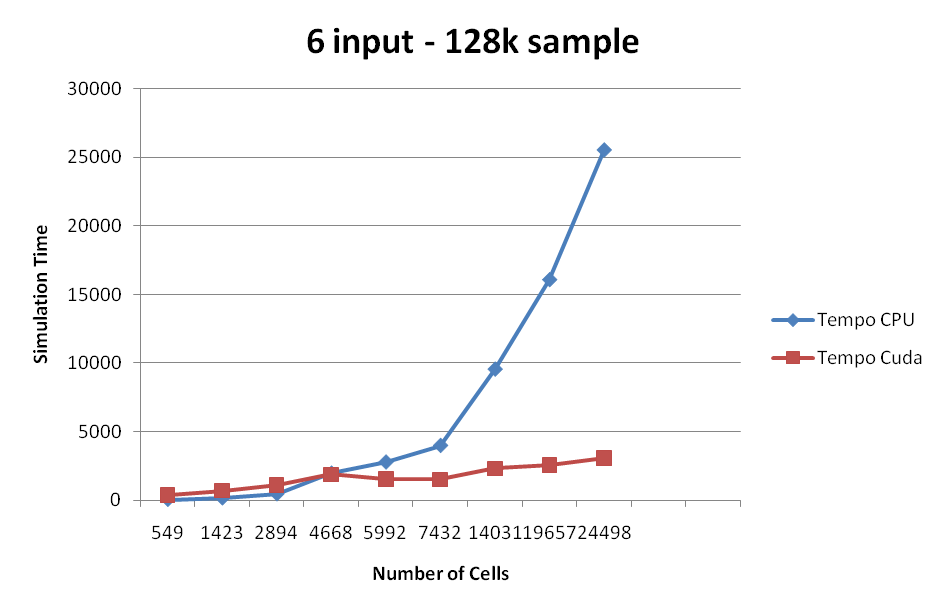
\includegraphics[scale=0.6]{img/graph5.png}
\label{graph5}
\end{figure}

The figure shows on the vertical axis the total simulation time. This time is the sum of the core simulation time and the preliminary phase. I our implementation the time spent in the preliminary phase is slight higher that the original time because of the coloring algorithm and the conversion to structures that are going to be allocated on the gpu.\newline
The simulation output obtained with the new implementation and the previous one are the same and are illustrated in the figure below. the difference of the output value in the initial samples are due to the circuit's latency illustrated in \ref{delay}. This is the output of a circuit with 3 inputs.

\begin{figure} [h!]
\centering
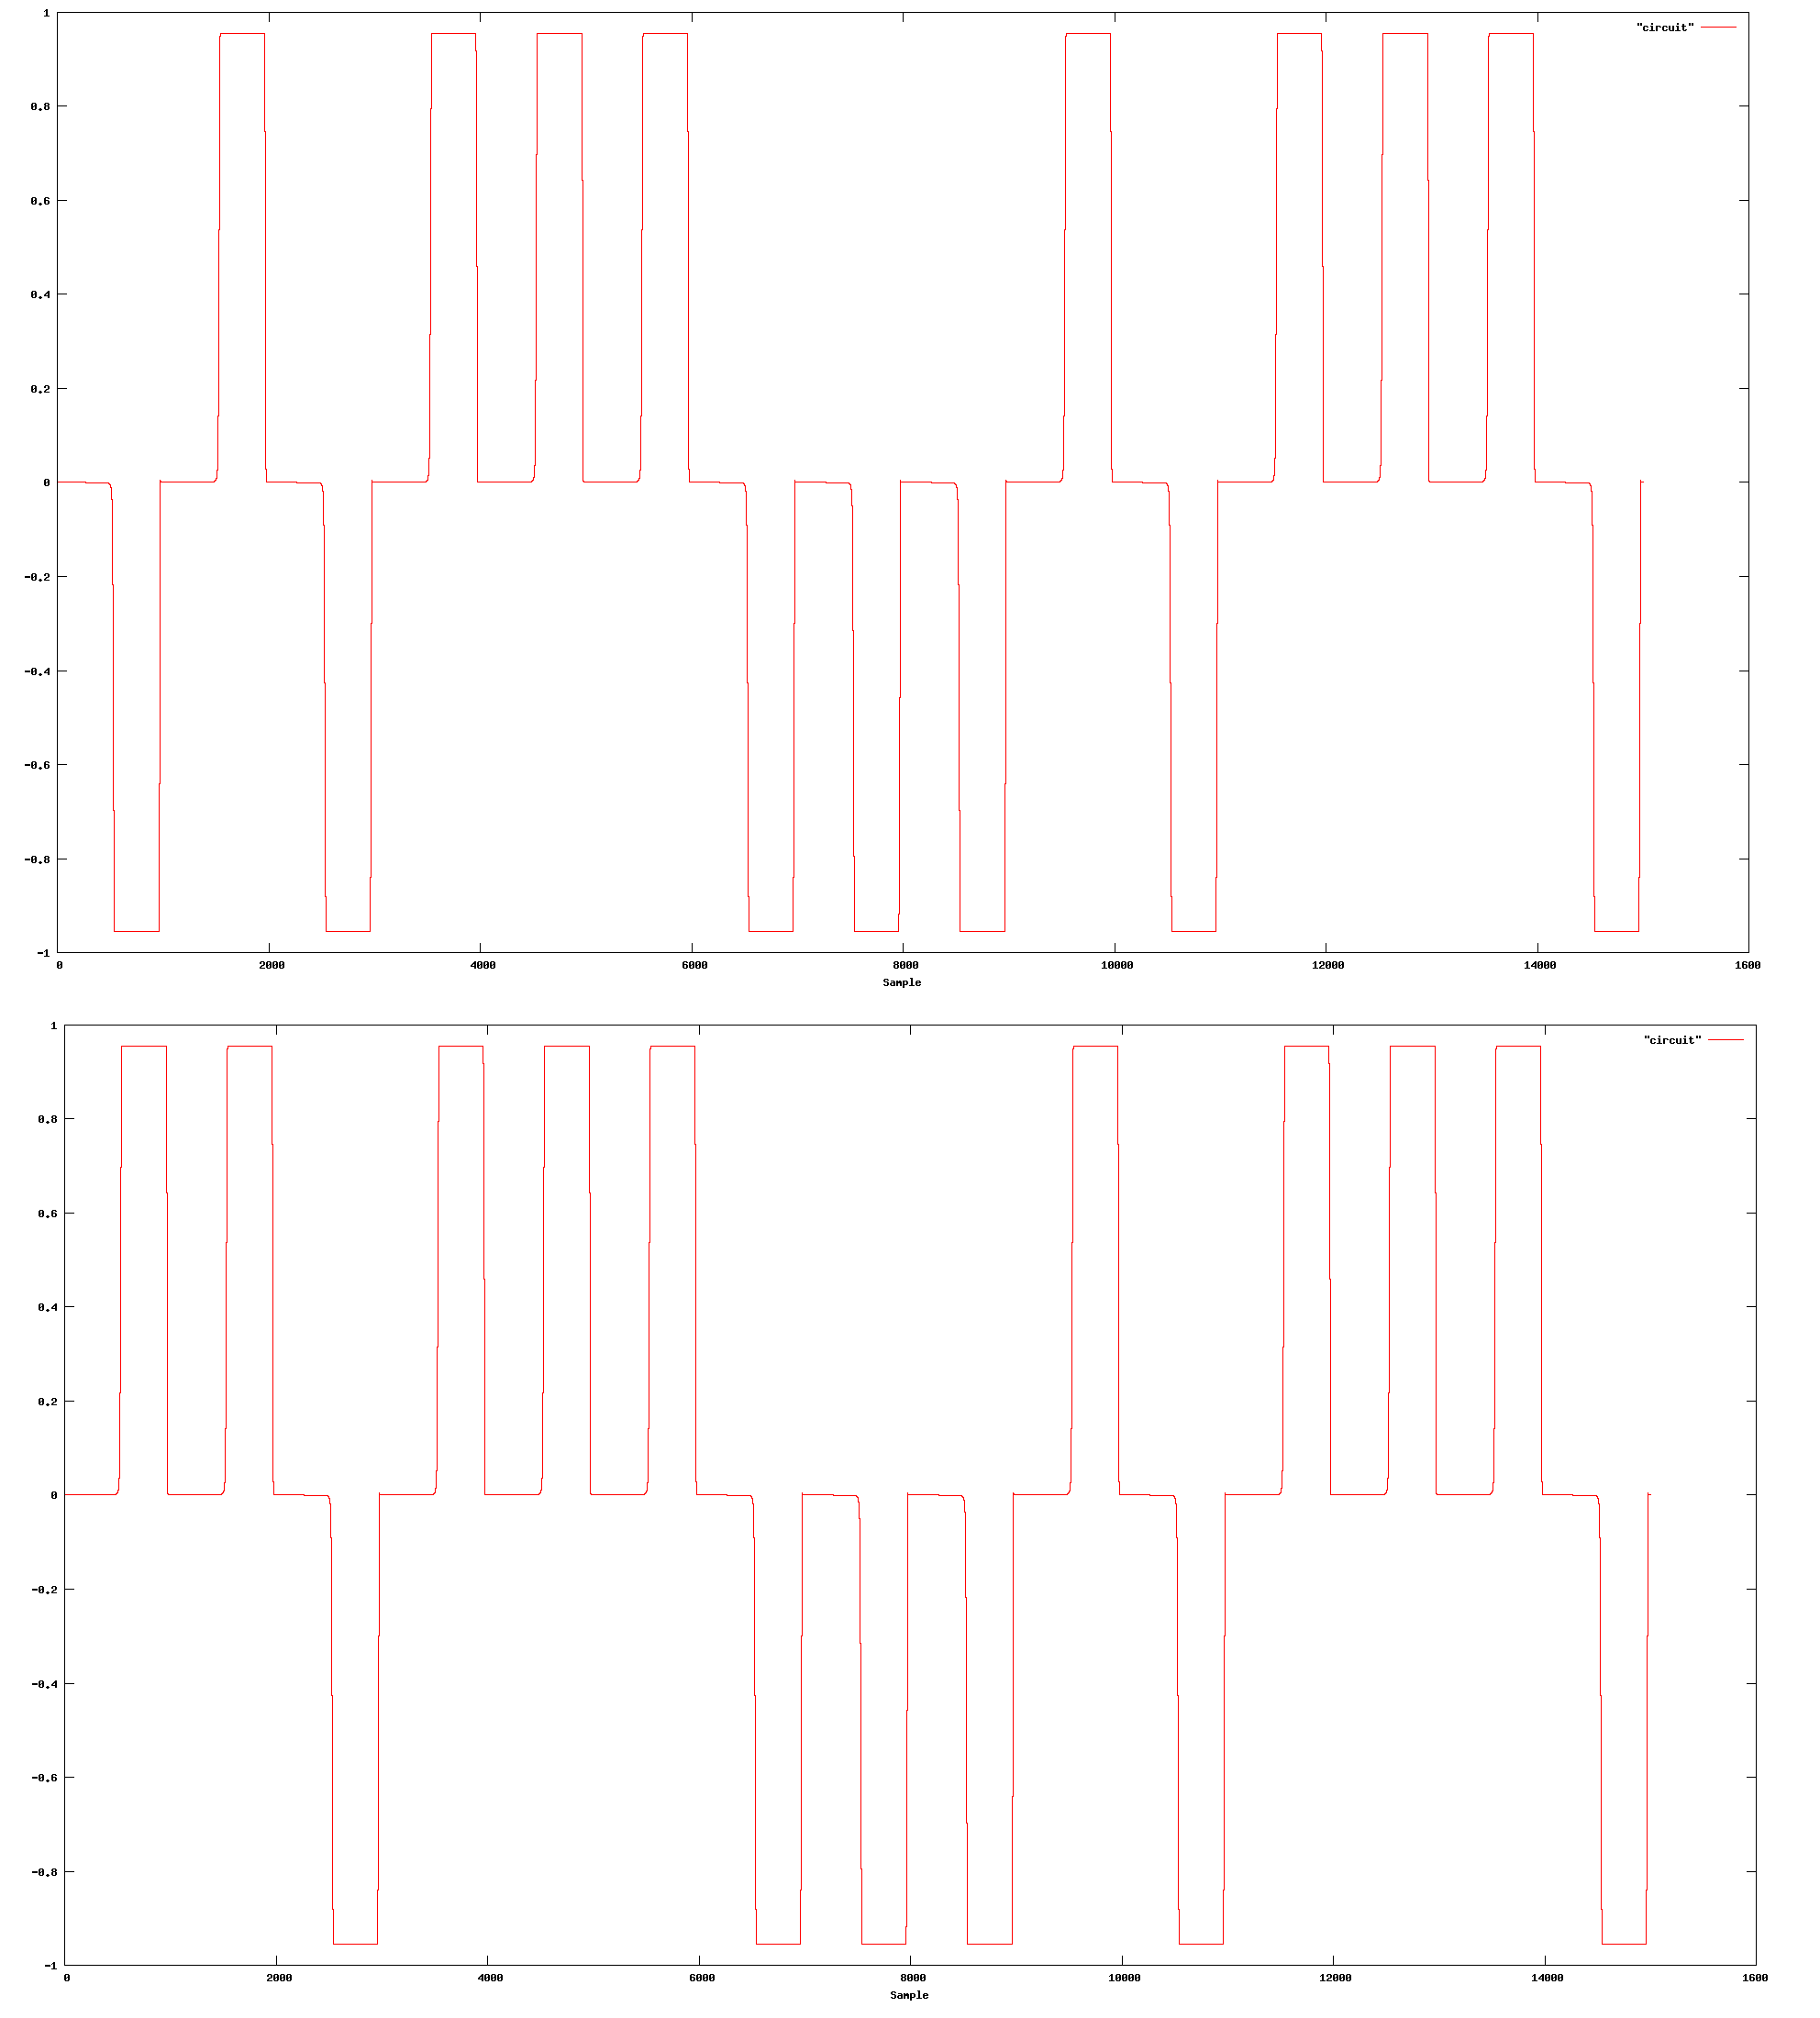
\includegraphics[scale=0.2]{img/result.png}
\label{graph5}
\end{figure}

The figures in the end of this document show the results of the simulations. The cpu simulations has been carried out on a system with a Xeon processor running at the speed of 2.0Ghz, the gpu simulations have been executed on a Tesla C1060. The figure below shows the speedup of the new implementation on the previous one. 

\begin{figure}
\centering
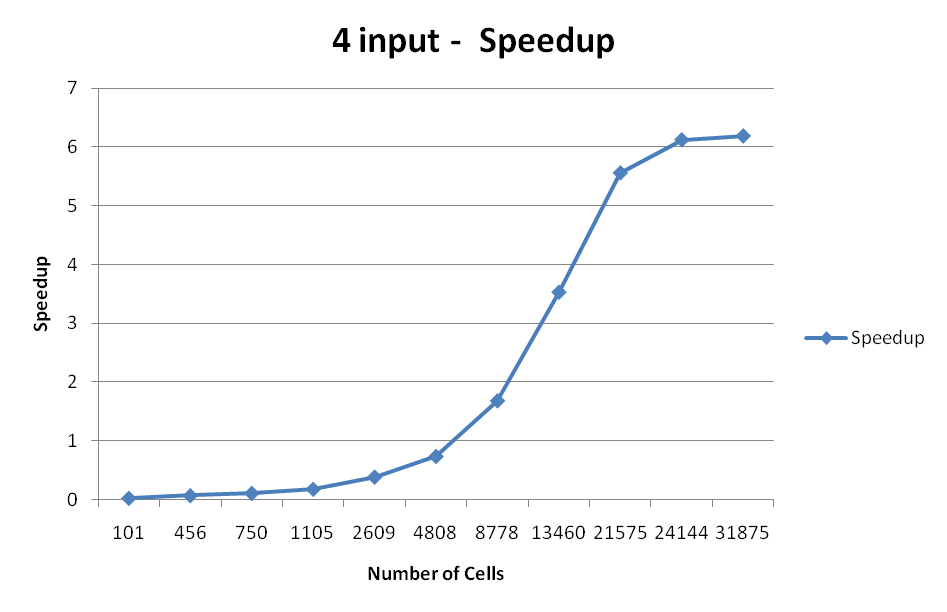
\includegraphics[scale=0.6]{img/speed.png}
\label{graph5}
\end{figure}

The initial speedup is very low and as expected it grows with the number of cells in the circuit. Over a certain number of cells the speedup meets superior limit. This limitation is due to the fact that the GPU can execute in parallel much less threads than the actual number of cells. This limitation force the GPU to serialize the execution of some threads. This is an intrinsic limitation of the architecture use for the simulation, not derived by the implementation. Using a GPU which allows more parallel threads will allow to raise this limit. The average speedup on the circuit with 4 inputs we have tested is of 2,2. The minimum speedup, which corresponds to the circuit with less cells is of 0,006 and the maximum is of 8,7.